% Copyright (C)  2015  Philipp Hacker.
% Permission is granted to copy, distribute and/or modify this document
% under the terms of the GNU Free Documentation License, Version 1.3
% or any later version published by the Free Software Foundation;
% with no Invariant Sections, no Front-Cover Texts, and no Back-Cover Texts.
% The lincense itself can be found at <https://www.gnu.org/licenses/fdl-1.3>.

\documentclass[numbers=noenddot,a4paper]{scrartcl}

\usepackage[greek,ngerman]{babel}
\usepackage[T1]{fontenc}
%\usepackage[applemac]{inputenc}
\usepackage[utf8]{inputenc}
\usepackage{fullpage}
\usepackage{scrpage2}
\usepackage{libertine}
%\usepackage{braket}
\usepackage{ziffer}
\usepackage{graphicx}
\usepackage{units}
\usepackage[infoshow]{tabularx}
\usepackage[all]{xy}
\usepackage{amsmath}
\usepackage{amssymb}
\usepackage{wrapfig}
\usepackage{upgreek}
\usepackage{esint}
\usepackage{float}
\usepackage[font=small,labelfont=bf]{caption}
\usepackage{subcaption}
\usepackage{lscape}
\usepackage[backref=page]{hyperref}
\usepackage{csquotes}
\usepackage[printonlyused,withpage,footnote]{acronym}

\renewcommand{\thefigure}{Abb. \arabic{figure}}
%\renewcommand{\bflabel}[1]{\normalfont{\normalsize{#1}}\hfill}

%\captionsetup[wrapfigure]{name=}
\captionsetup[figure]{name=}

\newcommand{\nummat}[1]{\left[\text{#1}\right]}
\newcommand{\num}[1]{$\left[\text{#1}\right]$}
\newcommand{\degree}{^\circ}
\newcommand{\diff}{\textnormal{d}}
\newcommand{\tenpo}[1]{ 10^{#1}}
\newcommand{\greek}[1]{\greektext#1\latintext}
\newcommand{\ix}[1]{_\text{#1}}
\newcommand{\imag}{\mathbf{i}}
\newcommand{\tilt}[1]{\textit{#1}}
\newcommand{\grad}[1]{\textit{grad}\left(#1\right)}
\newcommand{\divergenz}[1]{\textit{div}\left(#1\right)}
\newcommand{\euler}{\mathnormal{e}}
\newcommand{\fett}[1]{\textbf{#1}}

\title{Bachelor-Arbeit zum Thema \enquote{Modenanregung in \tilt{Yukawa}-Bällen}} %TODO Name
\author{Philipp Hacker} %TODO Author
\date{\today}

\setcounter{section}{-1}


\begin{document}
	
	\maketitle
	
	\begin{center}
		
		Institut für Physik\\
		mathematisch-naturwissenschaftliche Fakultät\\
		Universität Greifswald
		
	\end{center}
	 
	\vspace{0.5cm}
	
	\begin{figure}[H]
			\centering
			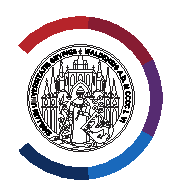
\includegraphics[width=0.35\textwidth]{figs/unilogo_NEU_schwarz.eps}
	\end{figure}
	
	\vspace{0.5cm}
	
	\begin{center}
			
			\hspace{-0.55cm} Erst-Gutachter: Prof. Dr. André Melzer \\ \vspace{0.25cm} %TODO Name Erst-Gutachter
			
			Zweit-Gutachter: Prof. Dr. Lutz Schweikhard \\ \vspace{0.25cm} %TODO Name Zweit-Gutachter
			
			Bearbeitungszeitraum: 01.03.2015 bis 12.07.2015 \\ \vspace{0.25cm} %TODO Bearbeitungszeitraum
		
%		\begin{table}[h]
%			\centering
%			Note (Erst-Gutachter): %TODO Gute Note erhalten :)
%			\begin{tabularx}{1.5cm}{|X|}
%				\hline \\ \\
%				\hline
%			\end{tabularx}
%			
%			\centering
%			\hspace{-0.42cm} Note (Zweit-Gutachter): %TODO Gute Note erhalten :)
%			\begin{tabularx}{1.5cm}{|X|}
%				\hline \\ \\
%				\hline
%			\end{tabularx}
%			
%		\end{table}

	\end{center}
	
	\thispagestyle{empty}
	
	\newpage
	
	\tableofcontents
	
	\newpage
	
	\section{Motivation}\label{sec:einleitung}
	
	\newpage
	
	\section{Physikalische Grundlagen}\label{sec:physg}
	
		\subsection{Grenzschichten von Plasmen}
		
			Die Grenzschichten zu Metallen von Plasmen sind dunkler, als die eigentliche Entladung. Dies ist auf einen Elektronenmangel zur\"uckruf\"uhren, da diese sonst im Hauptvolumen die Neutralgasatome zur Fluoreszenz anregen. Damit kann die Quasineutralit\"at der Entladung dort nicht mehr gelten und es entsteht eine positive Raumladungszone.\\
			Auf Grund der wesentlich gr\"o{\ss}eren Beweglichtkeit $\mu\ix{e}$ (wegen der kleineren Masse) und thermischen Geschwindigkeit $v\ix{th,e}$ der Elektronen wird eine Wand in einem Plasma h\"aufiger von diesen getroffen, als von den korrespondierenden Ionen. Betrachtet man nur die Oberfl\"ache dieser, so kann man annehmen, dass die Begrenzung einer Gasentlandung negativ aufgeladen ist. Das Potential, welches station\"ar unter dem Einfluss eines ``konstanten'' Plasmas wird, hei{\ss}t \tilt{floating}-Potential $\Phi{W,fl}$.
			
%				\begin{figure}
%					\centering
%					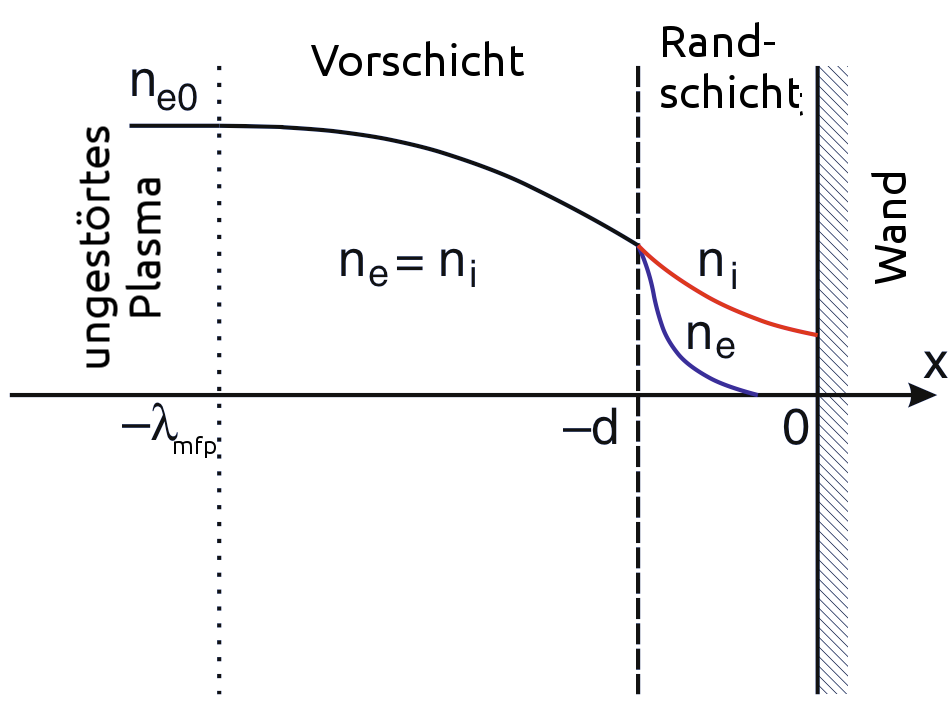
\includegraphics[]{randschichtpiel.png}
%					\caption{Schema der Dichteverl\"aufe an/in einer Plasmagrenzschicht. Im ungest\"orten Plasma liegen die Dichten $n\ix{e,0}=n\ix{I,0}$ vor; in der sog. Vorschicht fallen sie Bereits davon ab.
%					\label{img:randschicht}
%				\end{figure}

		\subsubsection{Child-Langmuir-Gesetz} \label{subsub:child-lang}
		
			Bla.	
			
		\subsubsection{Bohm-Kriterien}
		
			Es stellt sich u.a. die Frage, warum sich diese Randschicht, in der die Elektronendichte stark abnimmt und gegen die Grenze verschwindet, nicht in das gesamte Plasma durch eine R\"uckwirkung ausbreitet. Das hei{\ss}t also: Warum und wann ist die Randschicht(-grenze) stabil?\\
			Man stelle sich nun ein (mechanisches) Ein-Teilchen-Problem vor, bei welchem eine Gleichgewichtsanalyse vorgenommen wird. Das Potential habe ein Extremum - maximal oder minimal - an welchem die Punktmasse sich befindet. F\"ur die Behandlung des Randschicht-Problems sind nur Potentiale mit umgekehrt-parabelartigen Maxima interessant (siehe \ref{img:parab}), womit aus einer kleinen St\"orung eine gro{\ss}e Kraft auf das Teilchen folgt. In diesem Fall kann man also von einer Instabilit\"at sprechen.\\
			Der Bezug zur Plasmarandschicht wird deutlich, wenn man die Differentialgleichung des mechanischen Problems mit der Poissongleichung des Potentials in der Rand- bzw. Vorschicht - siehe Gl. (\ref{eq:pseudo}) vergleicht. Dabei stellt $\Psi\left(\Phi\right)$ ein Pseudopotential dar, welches in seiner Bedeutung vergleichbar mit der mechanischen Variante $V\left(\vec{r}\right)$ ist.
			
				\begin{align}
					m\frac{\diff^{2}\vec{r}}{\diff t^{2}}=-\frac{\diff V}{\diff\vec{r}} \Leftrightarrow \Delta_{\vec{r}}\,\Phi=-\frac{\diff\Psi}{\diff\Phi}=f\left(\Phi\right) \label{eq:pseudo}
				\end{align}
				
			Damit eine Instabilit\"at vorliegen kann, muss die, aus einer St\"orung des Pseudopotentials resultierende Kraft mit der Entfernung zum Gleichgewicht anwachsen. Die mathematisch \"aquivalente Formulierung ist Gleichung (\ref{eq:beding}). Nach Gl. (\ref{eq:pseudo}) und der in Abschnitt (\ref{subsub:child-lang}) hergeleiteten Dichten in der Grenzschicht, kann die geforderte Bedingung \"uberpr\"uft werden (siehe Gl. (\ref{eq:beding2})).
			
				\begin{align}
					\left.\frac{\diff^{2}\Psi}{\diff\Phi^{2}}\right|_{\Phi=0}<0 \label{eq:beding}
				\end{align}
				
%				\vspace{-0.3cm}
				
				\begin{align}
					\frac{\diff^{2} \Psi}{\diff\Phi^{2}}=&\frac{\diff f\left(\Phi\right)}{\diff \Phi}=\frac{\diff}{\diff\Phi}\left(\frac{\rho}{\epsilon\ix{0}}\right)=\frac{\diff}{\diff\Phi}\left(\frac{n\ix{e}\left(x\right)-n\ix{I}\left(x\right)}{\epsilon\ix{0}}\right) \nonumber \\
					=&\frac{en\ix{e}\left(-d\right)}{\epsilon\ix{0}}\left(\frac{e}{k\ix{b}T\ix{e}}\exp\left(\frac{e\Phi\left(x\right)}{k\ix{B}T\ix{e}}\right)-\frac{e}{m\ix{I}u\ix{0,I}^{2}}\left(1-\frac{2e\Phi\left(x\right)}{m\ix{I}u\ix{0,I}^{2}}\right)^{-\frac{3}{2}}\right) \label{eq:beding2} \\
					\Phi=0 \hspace{0.3cm} \Rightarrow  u\ix{0,I}\ge v\ix{B,I}=\sqrt{\frac{k\ix{B}T\ix{e}}{m\ix{I}}} \label{eq:bohmkriteins}
				\end{align}
				
		\subsection{Aufladung von Staubpartikeln}\label{subsec:ströme}
		
			Die Ladung eines Fremdteilchens (Staub) in einem Plasma ist eine dynamische Größe. Sie ist zeitlich veränderlich, als auch abhängig von den Plasmaparametern, den Partikeleigenschaften sowie dessen Trajektorie in der Entladung. Offensichtlich ergibt sich die Ladung eines Teilchens zum Zeitpunkt $t$ aus den Ladungsströmen $I\ix{k}$ der Plasmaspezies auf das Partikel bis zu diesem Zeitpunkt. Im folgenden genügt es, dieses Problem auf einer Zeitskala zu betrachten, in der man die Ladung als konstant unter dem Einfluss der Ströme annehmen kann. Damit werden diese ebenfalls stationär und es gilt für ein einzelnes Teilchens die \tilt{Kirchhoff'sche Knotenregel}, wobei der Staub ein Knoten sei:
			
				\begin{align}
					\sum_{\text{k}} I\ix{k}\left(\Phi\ix{fl}\right)=\frac{\diff Q\ix{S}}{\diff t} ß,\, . \label{eq:float}
				\end{align}

		Die Elektronen und Ionen im Plasma strömen aufgrund ihrer thermischen Bewegung auf das Fremdteilchen und verleihen diesem über Stöße eine Ladung $Q\ix{S}$, wobei sich für das Partikel ein elektrostatisches Potential $\Phi\ix{fl}$ einstellt, bei dem Gl. (\ref{eq:float}) gilt. Die Ladungsspezies kommen dabei im allgemeinen aus Sekundär-,Photo-, oder Feldemissionen, wobei die dominanten Ströme die des Plasmas selbst sind. Hier soll es ausreichen, die Plasmaströme nach  \tilt{Langmuir} und \tilt{Mott-Smith} mit dem sog. \tilt{orbital motion limit}-Modell \cite{Langmuir26} zu beschreiben. 
		
		\subsubsection{OML-Modell}\label{subsub:oml}
			
		Dabei wird angenommen, dass sich ein strömendes Teilchen, welches zu $Q\ix{S}$ beiträgt bzw. damit elektrostatisch wechselwirkt, stoßlos aus dem Unendlichen (durch die Entladung) darauf zu bewegen kann. Aufgrund der, im allgemeinen höheren Elektronentemperatur und -beweglichkeit wird $\Phi\ix{fl}<0$, woraus eine veränderte Wechselwirkung mit den Teilchen der Ladungsströme folgt. Man definiert folglich einen kritischen Stoßparameter $b\ix{k}$, welcher dem Abstand eines Ions zur Target-Achse entspricht, bei dem dieses durch die Coulomb-Anziehung des Partikels gerade noch dessen Oberfläche tangiert. Für Parameter $b>b\ix{k}$ wird ein eintreffendes Ion auf seiner Trajektorie nur abgelenkt, für $b<\ix{k}$ landet dieses auf dem Staubteilchen.\\
		Da vorausgesetzt wird, dass keine Stöße vor dem Target geschehen, kann die Impulserhaltung zusammen mit der Energieerhaltung für ein einzelnes Projektil aufgestellt werden, welches sich im Abstand $b\ix{k}$ darauf zu bewegt:
		
			\begin{align}
				|\vec{L}|=|\vec{r}\times\vec{p}|=m\ix{I}v\ix{I}a=m\ix{i}v\ix{i,0}b\ix{k} \label{eq:impulserhaltung} \\
				E\ix{I}=\frac{m\ix{I}}{2}v\ix{I}^2+e\Phi\ix{fl}=\frac{m\ix{I}}{2}v\ix{I,0}^2 \label{eq:energieerhaltung}
			\end{align}
			
		In Gl.(\ref{eq:impulserhaltung}) und (\ref{eq:energieerhaltung}) stehen jeweils die linken Seiten für den Zeitpunkt des Auftreffens und die rechten für das Einlaufen aus dem Unendlichen. Durch Umformungen lässt sich ein Ausdruck für den kritischen Stoßparameter, in Abhängigkeit vom Partikelradius und dem \tilt{floating}-Potential aufgestellt werden.
		
			\begin{align}
				b\ix{k}^2=a^2\left(1-\frac{e\Phi\ix{fl}}{\frac{m\ix{I}}{2}v\ix{I,0}^2}\right) \label{eq:krit}
			\end{align}
			
		Der zugehörige Streuquerschnitt für die Streuung eines Teilchenstroms an einem Staubpartikel wird damit zu $\sigma\ix{k}=\pi b\ix{k}^2$, welcher größer als die geometrische Querschnittsfläche $\pi a^2$.\\
		Der (differentielle) Ladungsträgerstrom $\diff I\ix{j}$, welcher schließlich den Parameter der Partikelladung bestimmt, ergibt sich aus der Aufsummierung aller Stromdichten von Teilchen der Geschwindigkeiten $v\ix{j}$, gewichtet mit ihren zugehörigen Wechselwirkungsquerschnitten $\sigma\ix{j}$ und (hier: maxwellartigen) Verteilungen $f\left(v\ix{j}\right)$:
		
			\begin{align}
				\diff I\ix{j}=\sigma\ix{j}&\left(v\ix{j}\right)n\ix{j}v\ix{j}f\left(v\ix{j}\right)\diff v\ix{j} \nonumber \\
				\text{Ionen: } I\ix{I}&=\pi a^2n\ix{I}e\sqrt{\frac{8k\ix{B}T\ix{I}}{\pi m\ix{I}}}\left(1-\frac{e\Phi\ix{P}}{k\ix{B}T\ix{I}}\right) \label{eq:ionenstrom} \\
				\text{Elektronen: } I\ix{e}&=-\pi a^2n\ix{e}e\sqrt{\frac{8k\ix{B}T\ix{e}}{\pi m\ix{e}}}\exp\left(\frac{e\Phi\ix{P}}{k\ix{B}T\ix{e}}\right) \label{eq:elektronenstrom}
			\end{align}
			
		($T\ix{e,I}$ - Elektronen-/Ionentemperatur; $n\ix{e,I}$ - Elektronen-/Ionendichte, $\Phi\ix{P}$ - Partikelpotential; $k\ix{B}$ - \tilt{Boltzmann}-Konstante )\\
		Der Unterschied zwischen Gl. (\ref{eq:ionenstrom}) und (\ref{eq:elektronenstrom}) resultiert aus den unterschiedlichen Arten der Wechselwirkung mit dem Staubteilchen. Da $\Phi\ix{P}<0$ ist, werden Ionen aller Geschwindigkeiten in Richtung des Partikels gelenkt und könnten theoretische damit stoßen (respektiv der Geschwindigkeitsverteilung und dem Streuquerschnitt). Die Elektronen hingegen müssen mindestens eine Geschwindigkeit $v\ix{min}=\sqrt{-\frac{2e\Phi\ix{P}}{m\ix{e}}}$ besitzen, damit sie die Potentialbarriere zum Partikel überwinden und damit stoßen können. Au{\ss}erdem finden sich mit $\sqrt{\frac{8k\ix{B}T\ix{j}}{\pi m\ix{j}}}$ die thermischen Geschwindikeiten der jeweiligen Spezies $j$ als Vorfaktoren wieder. Damit werden die Gesamtstr\"ome letztendlich zum Produkt aus ungest\"orter, thermischer Stromdichte und der angepassten Wechselwirkungsfl\"ache des Partikels. \\
		Es sei erwähnt, dass aufgrund der hohen Teilchendichten in einem Plasma die OML-Theorie nicht der Realität entspricht. Die mittlere freie Weglänge eines Ions oder Elektrons hat in etwa die Dimension der Debyelänge $\lambda\ix{D}$ und ist nicht, wie vorausgesetzt, unendlich groß. Des weiteren entsprechen die $f\left(v\ix{j}\right)$ in der Praxis nicht isotropen Maxwell-Geschwindigkeitsverteilungen.
		
		\subsubsection{Neutralgas-Ionen-Stöße}
		
		Auf Grundlage der OML-Theorie lässt sich ein erweiterter Ausdruck für den Ionenstrom mit Rücksicht auf Stöße des Neutralgases aufstellen. Offensichtlich geht, mit dem Durchgang eines Projektils durch das Neutralgas einer Entladung, der Verlust kinetischer Energie einher. Es ist nun leicht nachzuvollziehen, dass sich viele Ionen, aufgrund der Ablenkungen durch Stöße und Wechselwirkung, um das negativ geladene Staubpartikel sammeln.
		\\In einer Sphäre mit dem Radius $R$ um das Teilchen ist die Stoßwahrscheinlichkeit zwischen Ionen und Neutralgasatomen
		
			\begin{align}
				\frac{R}{l\lambda\ix{mfp}}=Rn\ix{N}\sigma\ix{I,N} \,\, . \label{eq:wahrschein}
			\end{align}
						
		($n\ix{N}$ - Neutralgasdichte; $\sigma\ix{I,N}$ - Stoßparameter für Ion-Neutralgas-Stöße; \mbox{$\lambda\ix{mfp}$ - mittlere freie Wegl\"ange})\\
		Durch eine Sph\"are mit diesem Radius flie{\ss}t nun neben dem thermischen Ionenstrom $I\ix{th}$ noch ein weiterer Strom $I\ix{S}$ auf Grund der St\"o{\ss}e mit dem Neutralgas. Die Ionen der Geschwindigkeit $v\ix{th,I}$, welche sich ohne Wechselwirkung mit dem Gas der Entladung am Target vorbei bewegen w\"urden, werden mit der Sto{\ss}wahrscheinlichkeit aus Gl. (\ref{eq:wahrschein}) in Richtung des Staubteilchens abgelenkt und tragen somit zum Ladungsstrom auf dieses bei. Der Gesamtladungsstrom durch Ionen entspricht der Summe der beiden Str\"ome:
		
			\begin{align}
				I\ix{th}=&\pi R^{2}n\ix{N}ev\ix{th,I} \quad I\ix{S}=\pi R^2n\ix{N}ev\ix{th,I}\left(Rn\ix{N}\sigma\ix{N,I}\right) \\
				&I\ix{ges}=\pi a^{2}n\ix{I}ev\ix{th,I}\left(1-\frac{e\Phi\ix{P}}{k\ix{B}T\ix{I}}+\frac{R^{3}}{\lambda\ix{mfp}a^{3}}\right)
			\end{align}
	
		Auf der Oberfl\"ache der '\tilt{Sto{\ss}sph\"are}' $\mathbb{S}\ix{R}$ hat das \tilt{Yukawa}-Potential des Staubteilchens gerade die Energie der thermischen Ionenbewegung (Gl. (\ref{eq:bestimmR})), womit diese gerade noch in dessen Einfang geraten. Mit dem daraus bestimmten $R$ folgt ein diskreter Ionenstrom auf das Partikel mit R\"ucksicht auf die Ionen-Neutralgaswechselwirkung (Gl. (\ref{eq:ionstromkorr})).
		
			\begin{align}
				\frac{k\ix{B}T\ix{I}}{e}=&\frac{Z\ix{S}e}{4\pi\epsilon\ix{0}R}\exp\left(\frac{R}{\lambda\ix{D}}\right) \label{eq:bestimmR} \\
				I\ix{I}=\pi a^{2} n\ix{I}e v\ix{th,I}&\left(1-\frac{e\Phi\ix{P}}{k\ix{B}T\ix{I}}+0,1\left(\frac{e\Phi\ix{P}}{k\ix{B}T\ix{I}}\right)^{2}\frac{\lambda\ix{D}}{\lambda\ix{mfp}}\right) \label{eq:ionstromkorr}
			\end{align}
			
		Im Vergleich zum Ergebnis des OML-Modells aus Gl. (\ref{eq:ionenstrom}) ist dieser Ladungstrom in Abh\"angikeit des Partikelpotentials und Ionentemperatur vergr\"o{\ss}ert. Die Wechselwirkung mit dem Neutralgas sorgt also, \"uber die St\"o{\ss}e und Erzeugung einer \tilt{Ionenwolke} um ein Teilchen, f\"ur einen gr\"o{\ss}eren pos. Ladungsstrom, welcher respektive wiederum f\"ur eine Steigerung des Elektronenstromes auf Grund des ver\"anderten Partikelpotentials sorgt. Eine selbstkonsistente L\"osung der, an den Anfang gestellte Problematik in Gl. (\ref{eq:float}) um das \tilt{floating}-Potential gestaltet sich jedoch als \"uberaus schwierig, da schon der OML-Theorie mehrere falsche Annahmen vorausgingen und dessen Eigenr\"uckwirkungen nicht-trivial sind.
			
		\subsection{Staub-Dynamik}\label{subsec:dynamik}
		
				In einem Plasma wirken viele, u.U. nicht-triviale Kräfte auf den eingefangenen Staub. Im Folgenden werden die wichtigsten Einflüsse auf die Dynamik komplexer Plasmen vorgestellt und beschrieben.\\
				\subsubsection{Gravitation und elektrische Feldstärke}\label{subsub:grav}
				
				Betrachtet man ein Experiment, welches am Erdboden in Nähe der Meereshöhe durchgeführt wird, so muss offensichtlich die vollständige Gravitationskraft berücksichtigt werden. Dies gilt bspw. nicht für Versuche unter Mikrogravitation während Parabelflügen oder auf der \tilt{International Space Station}.
				
					\begin{align}
						F\ix{g}=m\ix{S} g=\frac{4}{3}\pi a^3 \rho\ix{S} g
					\end{align}
				
				($m\ix{S}$ - Masse der Staubteilchen; $a$ - Partikelradius; $\rho\ix{S}$ - Massendichte des Staubes; $g$ - \mbox{Erdbeschleunigung})\\
				Natürlich wirkt auf die, durch das ionisierte Gas elektrisch geladenen Partikel eine elektrische Kraft $F\ix{E}$, welche aus dem äußeren Feld $E$ der Plasma-Elektroden folgt. Eine elektrische Wechselwirkung mit dem Plasma tritt aufgrund der Quasineutralität nicht auf: innerhalb einer \tilt{Debye-Kugel} sind die Veränderung zu schnell, als dass das träge Staubteilchen diesen folgen könnte. 
				
					\begin{align}
					F\ix{E}=Q\ix{S} E=4 \pi \epsilon\ix{0} a \Phi\ix{fl} E
					\end{align}
		
				($Q\ix{S}$ - Staubladung; $\Phi\ix{fl}$ - \tilt{floating}-Potential)\\
				Diese beiden Kräfte heben sich gerade in der Randschicht einer sog. Radiofrequenz-Entladung (\tilt{rf discharge}) auf, da sie für eine oben liegende Kathode antiparallel stehen. Zu beachten ist hierbei der stark unterschiedliche Einfluss des Teilchenradius - $\propto a^3$ und $\propto a$.\\
								
				\subsubsection{Abschirmung und Polarisationskräfte}\label{subsub:abschirm}
				
				Die große negative Aufladung der Staubteilchen sorgt über die Coulomb-Wechselwirkung mit den auf das Partikel zuströmenden Ionen dafür, das sich eine Konzentration derer lokal stark ändert. Es entsteht eine Wolke aus langsamen Ionen die quasi in der näheren Umgebung um das Teilchen verbleiben, jedoch nicht mit diesem interagiert und es nach außen hin vor dem Einfall schnellerer pos. Ladungen abschirmen. Somit gibt es keine direkte Rückwirkung der Wolke auf das Partikel, sofern dessen sphärische Symmetrie gegeben ist. Gilt dies nicht, so entsteht ein Multipol- bzw. Dipolmoment $\vec{p}$, welches danach strebt, sich in Richtung des Feldes $\vec{E}$ auszurichten. Damit wirkt eine Kraft $F\ix{Dip}$ (für ein Dipolmoment) auf das Staubteilchen zurück, welche mit dem Gradienten der Richtungsdifferenz zwischen $\vec{p}$ und $\vec{E}$ geht.

					\begin{align}
						\centering
						\vec{F}\ix{Dip}&=\vec{\nabla}\left(\vec{p}\vec{E}\right)\\
						&{\overset{\vec{p}\,||\vec{E}}{=}}\grad{pE} \nonumber
					\end{align}
					
				Das besagte Dipolmoment entsteht u.a. durch die diversen, gerichteten Ladungsprozesse in dem Plasma. Ein Partikel, welches in der Randschicht eingefangen und von einer Ionenwolke umgeben wird, 'sieht' unterschiedliche \tilt{Debye}-Längen über und unter sich aufgrund der lokalen Feldrichtung und der stark vom Mittelwert abweichenden Ionen- und Elektronendichten. Somit ändert sich offensichtlich die Plasmadichte innerhalb des Volumens einer Kugel mit dem, nun ortsabhängigen Radius $\lambda\ix{D}\left(\vec{r}\right)$. Insgesamt folgt daraus eine neue Bestimmungsgleichung für das Potential und damit auch eine neue Kraft $F\ix{E}$.
				
					\begin{align}
						\Delta \Phi\left(\vec{r}\right)-\frac{\Phi\left(\vec{r}\right)}{\lambda\ix{D}^2\left(\vec{r}\right)}=\frac{Q\ix{s}}{\epsilon\ix{0}}\delta\left(\vec{r}\right) \\
						F\ix{E}=\underbrace{Q\ix{S}E}_{\text{(I)}}-\underbrace{\frac{Q\ix{S}^2}{8\pi\epsilon\ix{0}}\frac{\nabla\lambda\ix{D}\left(\vec{r}\right)}{\lambda\ix{D}^2}}_{\text{(II)}}
					\end{align}
				
				Hierbei stellt (I) die normale Komponente dar und (II) ist zusätzliche Kraft durch die Deformation der Ionenwolke in Richtung kleinerer \tilt{Debye}-Längen $\lambda\ix{D}\left(\vec{r}\right)$. Die Kraft $F\ix{E}$ kann also dadurch größer oder kleiner werden. Hinzu kommt, dass der veränderte Parameter $\lambda\ix{D}$ von der Driftgeschwindigkeit $u\ix{I}$ abhängt, welche die Ionenwolke maßgeblich beeinflusst. Ist jedoch $u\ix{I}<v\ix{th,I}$ so kann man annehmen, dass die Ionenwolke besteht und $\lambda\ix{D}\left(\vec{r}\right)\approx\lambda\ix{D,I}$ gilt.\\
				Sind die Ionen jedoch schneller, womit $u\ix{I}>>v\ix{th,I}$ wird, so können sie nicht mehr vom Feld des Partikels 'gefangen' werden und damit die Ionenwolke bilden. So gilt folglich $\lambda\ix{D}\left(\vec{r}\right)\approx\lambda\ix{D,e}$.\\
				Insgesamt ist der Einfluss der Polarisation vernachlässigbar klein, solange die Teilchen eine Größe von einigen hundert $\unit{\mu m}$ nicht übersteigen.

			\subsubsection{Ionen-Neutralgasreibung}\label{subsub:reibung}

				Aufgrund der hohen negativen Ladung des Staubteilchens und der daraus resultierenden elektrostatischen Wechselwirkung existiert ein, relativ auf das Partikel zufließender, Ionenstrom oder auch "`Ionenwind"'. Weiterhin bewegen sich mit ihrer thermischen Geschwindigkeit die Neutralgasatome durch das Plasma und stoßen mit anderen Teilchen. Die Zahl der Stöße $\diff N$ einer Spezies mit einem Target mit dem Streuparameter $\sigma$ im Zeitintervall $\diff t$ ist somit über deren relative Geschwindigkeit $v\ix{rel}$ zu diesem in $\diff N=n\sigma v\ix{rel}\diff t$ gegeben. Hierbei kennzeichnet $n$ die Stromdichte der strömenden Teilchen. Aus diesem Strom folgt ein gewisser Impulsübertrag $\Delta p$ auf das Target. Hieraus lässt sich eine Kraft $F\ix{drag}$ ziehen, die einer Reibung bzw. einer Impulsaufnahme entspricht.
				
					\begin{align}
						F\ix{drag}=\frac{\diff N \Delta p}{\diff t}=\Delta p n \sigma v\ix{rel}
					\end{align}
					
				Man spricht hierbei auch von \tilt{ambipolarer Diffusion}, da die Ionenströme und damit auch die Ionenreibung zu beiden Polen führen. Man kann diese aus 2 Teilen aufbauen: direkte Kollisionen mit den Ionen $F\ix{dir}$ und deren Coulomb-Streuung an den Feldern der neg. geladenen Staubpartikel. Im folgenden soll das sog. \tilt{Barnes-Modell} eingeführt werden, welches die besagte Ionenreibung beschreibt.
				
				\paragraph{Ionenreibung: \tilt{Barnes-Modell}}
				
				Für die Bestimmung von $F\ix{dir}$ wird angenommen, dass nur die Ionen, welche für eine Ladungsänderung der Partikel sorgen, auch diese direkt treffen. Im Rückblick auf die Bestimmung der Ionenströme in \ref{subsec:ströme} wird die Kraft durch Kollisionen zu
				
					\begin{align}
						F\ix{dir}=\pi a^2m\ix{I}\tilde{v}n\ix{I}u\ix{I}\left(1-\frac{2e\Phi\ix{fl}}{m\ix{I}\tilde{v}^2}\right)\,\,.
					\end{align}
					
				($n\ix{I}$ - Ionenkonzentration; $u\ix{I}$ - Ionen-Driftgeschwindigkeit; $m\ix{I}$ - Ionenmasse)\\
				Das Produkt aus Masse und mittlerer Geschwindigkeit der Ionen $m\ix{I}\tilde{v}=m\ix{I}\sqrt{u\ix{I}^2+v\ix{th,I}^2}$ entspricht dem Impulsübertrag.\\
				Für die Coulomb-Streuung müssen alle diejenigen Ionen miteinbezogen werden, welche mit dem Feld des Staubes 'stoßen'. Hierfür wird der Streuquerschnitt $\tilde{\sigma}$ der Ionen-Elektronen-Wechselwirkung auf den aktuellen Fall angepasst.
				
					\begin{align}
						\tilde{\sigma}=4\pi b_{\frac{\pi}{2}}^2\ln\left(\Lambda\right)=&\,4\pi b_{\frac{\pi}{2}}^2\ln\left(\frac{\lambda\ix{D}}{b_{\frac{\pi}{2}}}\right) \\
						b_{\frac{\pi}{2}}=&\,\frac{e^2}{4\pi\epsilon\ix{0}m\ix{I}v^2} \nonumber
					\end{align}
					
				Der Stoßparameter $b_{\frac{\pi}{2}}$ beschreibt eine Ablenkung um $\unit[90]{\degree}$. Für die Ionenreibung müssen weitere Bedingungen mit eingebunden werden: die Coulomb-Streuung außerhalb der Ionenwolke ist irrelevant, die Staubpartikel haben eine endliche Ausdehnung und damit existiert ein minimaler Stoßparameter $b\ix{k}$. Damit wird das gesuchte $\sigma$ zu
				
					\begin{align}
						\sigma=\int_{b\ix{k}}^{\lambda\ix{D}}\tilde{\sigma}\diff\left(\frac{\lambda\ix{D}}{b_{\frac{\pi}{2}}}\right)=&\,4\pi b_{\frac{\pi}{2}}^2\ln\left(\frac{\lambda\ix{D}^2+b_{\frac{\pi}{2}}^2}{b\ix{k}^2+b_{\frac{\pi}{2}}^2}\right)^{1/2} \nonumber \\
						F\ix{Coul}\overset{*}{=}&\,\frac{2\pi a^2 e^2\Phi\ix{fl}^2}{m\ix{I}\tilde{v}^3}n\ix{I}u\ix{I}\ln\left(\frac{\lambda\ix{D}^2+b_{\frac{\pi}{2}}^2}{b\ix{k}^2+b_{\frac{\pi}{2}}^2}\right)^{1/2} \, \, .
					\end{align}
					
				Wobei in * für die vollständige Coulomb-Kraft durch Ionen $F\ix{Coul}$ auf ein Partikel benutzt wurde, dass dieses mit Ladung $Z\ix{S}e=Q\ix{S}$ als Kugelkondensator als $Q\ix{S}=4\pi\epsilon\ix{0}a\Phi\ix{fl}$ ausgedrückt werden kann. Wichtig zu beachten ist jedoch, dass nur Ionen einen Beitrag leisten, die innerhalb eines Stoßparameters $\lambda\ix{D}\approx\lambda\ix{D,e}$ am \tilt{target} vorbei fliegen.\\
				Die gesamte Kraft durch Ionen auf die Staubteilchen ist somit die Summe der Kräfte aus direkten Stößen und Coulomb-Kollisionen $F\ix{ion}=F\ix{dir}+F\ix{Coul}$, welche zusammen dargestellt sind in \ref{img:ionkräfte}.
				
					\begin{figure}
						\centering
						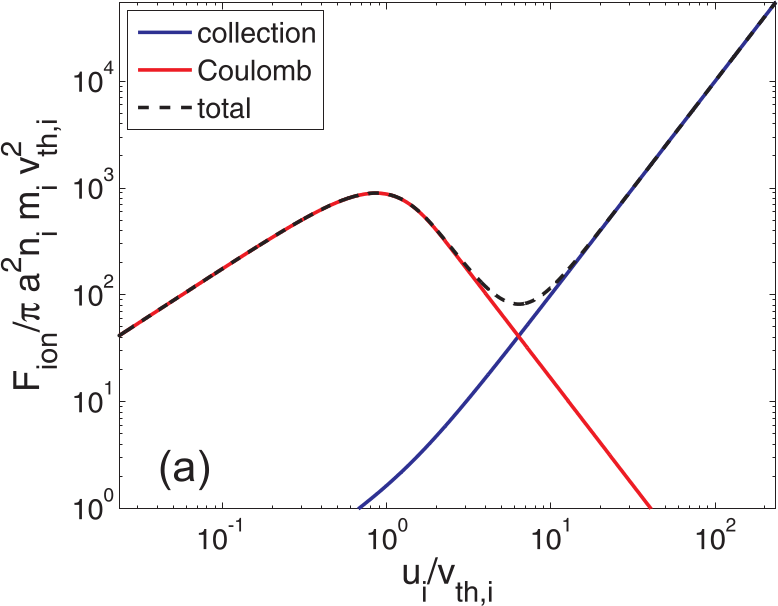
\includegraphics[height=0.4\textwidth,width=0.6\textwidth]{figs/forcesandtrappingmelzer.png}
						\caption{Berechnete Kräfte $F\ix{Coul}$ (\tilt{Coulomb}), $F\ix{dir}$ (\tilt{collection}) und die Summe beider auf einer doppelt-logarithmischen Skala.}\label{img:ionkräfte}
					\end{figure}
					
			\subsubsection{Neutralgasreibung}
			
				Die Stöße mit den Neutralgasatomen können, ebenso wie die mit Ionen, als Kraft durch Reibung aufgefasst werden. Diese sorgen insbesondere für eine Verlangsamung der Bewegung der Staubteilchen. Die Kraft $F\ix{N}$ wird, in ähnlicher Weise wie $F\ix{dir}$, durch einen Impulsübertrag über einen Strom von Neutralgasteilchen auf einen effektiven Querschnitt ausgedrückt.
				
					\begin{align}
						F\ix{N}=-\delta\frac{4}{3}\pi a^3m\ix{N}v\ix{th,N}n\ix{N}v\ix{S}
					\end{align}
					
				($m\ix{N}$ - Neutralgasatommasse; $v\ix{th,N}$ - thermische Geschw. der Neutralgasatome; $n\ix{N}$ - Neutralgasdichte; $v\ix{S}$ - Staubteilchengeschw.)\\
				Der Faktor $\delta$ beschreibt hierbei die Art, wie die Neutralgasatome mit dem Staub stoßen. Eine spiegelnde Reflexion tritt für ein $\delta=1$ auf. Mit steigendem $\delta$ wird die Kollision immer diffuser, bis hin zu einem Wert von $\delta=1,44$.\\
				Für den berühmten \tilt{Milikan}-Öltropfen-Versuch zur Bestimmung der Ladung eines Elektrons wurde, 1924 von \tilt{P. S. Epstein}, ebenso ein Ausdruck für die Kraft durch Neutralgasreibung bestimmt. Dabei ist $\beta$ der Reibungskoeffiziént und $\rho\ix{S}$ die Dichte des Staubmediums.
				
					\begin{align}
						F\ix{N}=-m\ix{S}\beta v\ix{S}=-m\ix{S}v\ix{S}\delta\frac{8}{\pi}\frac{p}{a\rho\ix{S}v\ix{th,N}}
					\end{align}
					
			\subsubsection{Thermophoretische Kraft}\label{subsub:therm}
	
				In einer Plasmakammer kann, durch Aufheizung oder Abkühlung einer der Elektroden bzw. Kammerbegrenzungen ein, bspw. der Gravitation oder dem elektrischen Feld entgegen gerichteter Temperaturgradient angelegt werden.\\
				Die Kraft kann folgendermaßen erklärt werden: auf der Seite der höheren Temperatur haben die Neutralgasteilchen im Mittel eine größere Geschwindigkeit und Impuls, woraus ein positiver Impulsübertrag in Richtung niedrigerer Temperaturen folgt.	Mit der Wärmeleitfähigkeit des Neutralgases $\kappa\ix{N}$ folgt für die thermophoretische Kraft $F\ix{th}$ Gl. (\ref{eq:therm}). Auf Grund $\propto a^2$ ist diese Kraft besonders wichtig für Teilchen mit einem Radius kleiner als $\unit{\mu m}$. Sie wird für die Formation von sog. \tilt{Yukawa-Clustern} genutzt (siehe \ref{subsec:yukawaclust}).
				
					\begin{align}
						F\ix{th}=-\frac{32}{15}\frac{a^2 \kappa\ix{N}}{v\ix{th,N}}\grad{T} \label{eq:therm}
					\end{align}
					
				Es sei erwähnt -  über die Zustandsgleichung für ideale Gase $pV=Nk\ix{B}T$ ersichtlich -, dass bei einer höheren Temperatur die Dichte des Neutralgases sinkt. Experimentell findet man daher, dass die verminderte Dichte zu einer niedrigeren Stoßintensität führt und damit den Effekt der Thermophorese in etwa gerade kompensiert. Trotzdem bleibt die Methode des Temperaturgradienten ein wichtiges Mittel zum Einfang des Staubes und Ausgleich der Gravitationskraft.
					
			\subsubsection{Kraft durch \tilt{Laser}-Einstrahlung}
			
				Der Einsatz von \tilt{Laser} (\fett{L}ight \fett{A}mplification by \fett{S}timulated \fett{E}mission of \fett{R}adiation) hat in Versuchen zu kolloidalen Plasmen verschiedene Gründe: einerseits wird der \tilt{target}-Bereich mit ihnen ausgeleuchtet, andererseits können unterschiedliche dynamische Eigenschaften des Staubes untersucht werden.\\
				Die Manipulation von eingefangenen Teilchen wird bspw. durch die Fokussierung eines \tilt{Laser}strahls auf ein Partikel realisiert. Hierbei spielt der Impulsübertrag der Photonen mit Impuls $p\ix{Ph}$, welcher dem Strahlungsdruck $p\ix{Strahl}$ entspricht und die photophoretische Kraft $F\ix{ph}$ eine Rolle.
				
					\begin{align}
						p\ix{Strahl}=\frac{\diff p\ix{ph}}{A\ix{L}\diff t}=&\frac{\diff N\ix{ph}}{A\ix{La}\diff t}\frac{h}{\lambda}=\frac{I\ix{L}}{c} \nonumber \\
						F\ix{Strahl}=&\gamma\frac{I}{c}\pi a^2 \label{eq:strahl}
					\end{align}
					
				($N\ix{ph}$ - Anzahl der, die das Partikel treffenden Photonen; $\lambda$,$\nu$ - Lasergrößen; $A\ix{L}$ - Querschnittsfläche des \tilt{Laser}; $\gamma$ - Wechselwirkungskoeffizient für den Stoß Photon-Staub)\\
				Für ein $\gamma=2$ in Gl. (\ref{eq:strahl}) liegt eine Totalreflexion vor, für $\gamma=1$ wird der Impuls der auftreffenden Photonen vollständig absorbiert.\\
				Geht man davon, dass die Photonendichte nicht isotrop über die Querschnittsfläche $A\ix{L}$ ist, so existiert ein Intensitätsgradient über die Strecke eines Strahlradius. Somit treten innerhalb der Strahlungsfläche auf ein Partikel unterschiedliche Kräfte durch den \tilt{Laser} auf: im Mittel treffen mehr Photonen das Partikel auf der Seite, welcher dem Strahlmittelpunkt zugewandt ist, als auf der entgegengesetzten. Somit entsteht eine Kraft, welche senkrecht auf der \tilt{Laser}-Richtung steht und zum Strahllot zeigt. Ein \tilt{Laser}-Strahl kann also zum Einfang von (einem) ausgewählten Partikeln benutzt werden.\\
				Bei der photophoretischen Kraft wird die resultierende Dynamik aus dem, durch die Stöße mit Photonen erzeugten Temperaturgradienten über ein einzelnes Partikel beschrieben. Wie bereits erläutert, liegt ein Strahldichtegradient für eine Fläche von $A\ix{S}$ vor, woraus eine unterschiedliche Staubaufheizung durch die Stoßreibung folgt.\\
				Treffen nun Neutralgasatome auf die heißere Seite, so werden sie dort schneller reflektiert, als von der kälteren. Die Differenz des Impulsübertrags resultiert in der photophoretischen Kraft, die entgegen des Gradienten der Photonendichte und damit in Richtung der heißen Seite der Partikel zeigt. Je nach der Absorptionsfähigkeit besitzen die Teilchen unterschiedliche Temperaturgradienten. Somit stellt sich eine heiße Front aus den Teilchen auf, welche eine gute Absorption und somit insgesamt höhere Temperatur aufweisen. Für diese Partikel zeigt $F\ix{ph}$ in Richtung des Strahls. Analog wirkt die photophoretische Kraft für schlecht absorbierende Teilchen in entgegengesetzte Richtung. Somit ergibt sich $F\ix{ph}$ in Gl. (\ref{eq:photoph}) mit dem Wärmeleitungskoeffizienten $\kappa\ix{S}$ des Staubes, dem Gasdruck $p$ und der Gastemperatur $T$.
				
					\begin{align}
						F\ix{ph}=\frac{\pi a^2 p I\ix{L}}{6\left(pav\ix{th,n}+\kappa\ix{S}T\right)} \label{eq:photoph}
					\end{align}
				
			\subsubsection{Einfang und Gleichgewicht}
			
				In \ref{img:kräfte} sind einige der bisher beschriebenen Kräfte für typische Parameter berechnet und mit einer doppelt-logarithmischen Skala dargestellt worden.\\
				Für Teilchen mit einem Radius im Bereich von einigen $\unit{\mu m}$ sind die Kräfte des äußeren elektrischen Feldes $F\ix{E}$ und der Gravitation $F\ix{G}$ dominant. Daher müssen, für einen praktikablen Einfang, diese beiden Kräfte im Gleichgewicht sein, d.h. sich stationär aufheben. Dies ist gerade in der nahen Randschicht der positiven Elektrode der Fall, da dort $F\ix{E}$ stark genug ist. Weil $\grad{E}\ll1$ ist, gilt dies nur lokal.\\
				Für $a\gg\unit[1]{\mu m}$ wird $F\ix{E}$ weniger relevant und es übt die Thermophorese eine immer größere Kraft auf den Staub aus. Genauer: $F\ix{th}$ ist in Experimenten sogar schon für $\grad{T}\approx \unit[2]{\frac{K}{m}}$ eine wichtige, nicht vernachlässigbare Größe. Für die Neutralgasreibung $F\ix{N}$ gilt, dass diese bei großen thermischen Geschwindigkeiten des Staubes nahezu konstant wird, jedoch für "`kalten"' Staub mit zunehmendem Drift $v\ix{S}$ an Einfluss gewinnt. Die Ionenreibung $F\ix{ion}$ ist unter diesen Umständen vergleichsweise klein.\\
				Sind die Staubpartikel klein, d.h. haben einen Radius $a\approx\unit[\tenpo{-9}]{m}$, so wird die Gravitationskraft mit ihrem Einfluss $\propto a^3$ sehr klein und spielt damit kaum noch eine Rolle. Damit muss die Kraft des elektrischen Feldes mit der Ionenreibung bzw. der Thermophorese balanciert werden.		
						
					\begin{figure}
						\centering
						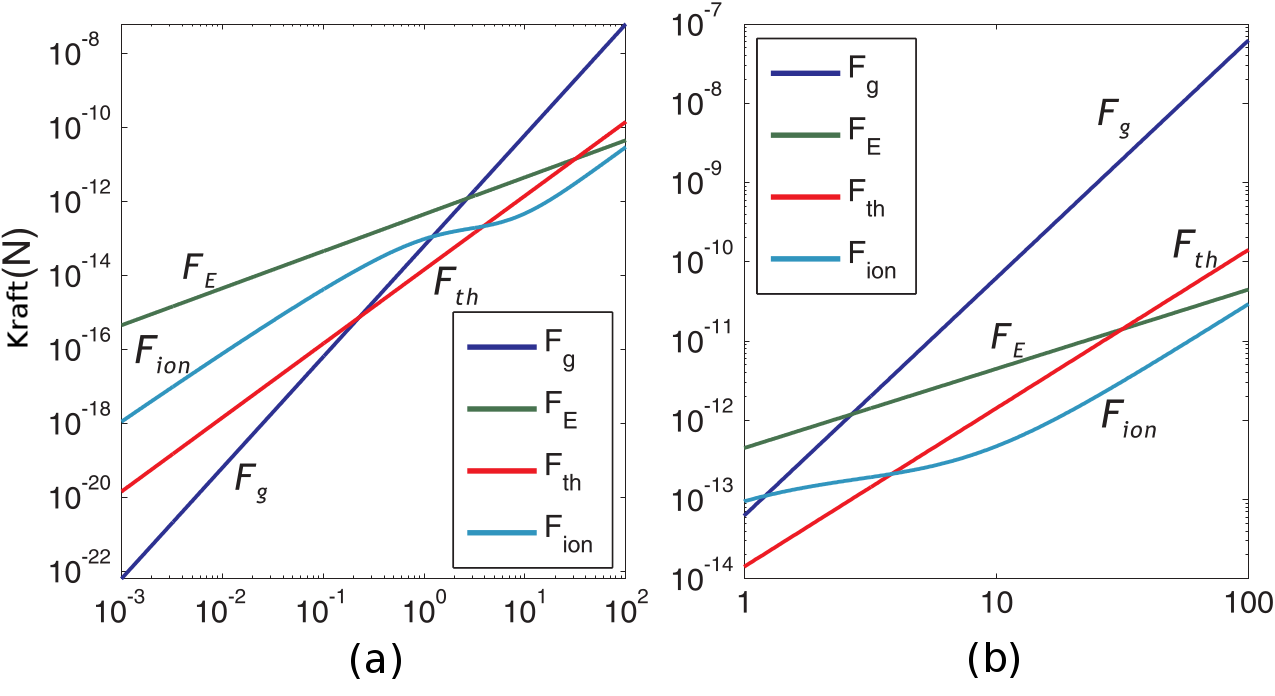
\includegraphics[width=1\textwidth,height=0.5\textwidth]{figs/allforcesequlibriummelzer.png}
						\caption{Kräfte als Funktion des Teilchenradius in einem Argon-Plasma (Parameter: $\kappa\ix{N}=\unit[0,016]{\frac{kg m}{s^3}}$;  \mbox{$\rho\ix{S}=\unit[1,5\cdot\tenpo{3}]{\frac{kg}{m^3}}$}; $T\ix{e}=\unit[2]{eV}$; $\Phi\ix{fl}=\unit[-4]{V}$; $E=\unit[1000]{\frac{V}{m}}$; $n\ix{I}=\unit[\tenpo{5}]{m^{-3}}$; $u\ix{I}=v\ix{th,I}=v\ix{th,N}=\unit[400]{\frac{m}{s}}$)} \label{img:kräfte}
					\end{figure}
				
				In \ref{img:kräfterichtungen} sind schematisch die Kräfte aus \ref{img:kräfte} mit ihren Orientierungen dargestellt worden. \\
				Abbildungsteil (a) zeigt dabei den Einfang von $\unit{\mu m}$-großen Teilchen in einer kleinen, lokalisierten Randschicht. Diese ordnen sich dabei in ausgedehnten Schichten mit hexagonaler Struktur (\tilt{fcc} bzw. \tilt{bcc}, siehe \ref{subsec:coulombkristall}) an. Die Kräfte der Thermophorese und des "`Ionenwindes"' ($F\ix{ion}$) zeigen dabei aus dem Plasma heraus in Richtung der Kammer bzw. der Elektroden. Hierbei sind die Ionen bestrebt, aufgrund der ambipolaren Diffusion in der Randschicht auf die Kammerwand, den Ladungsunterschied (etwa innerhalb einer \tilt{Debye}-Länge) zwischen dem Plasma und dem Gehäuse auszugleichen. Das liegt u.a. an den unterschiedlichen Beweglichkeiten der Ladungsträger und deren Strömung auf die Kammer. Weiterhin gilt ähnliches für die thermophoretische Kraft: das aufgeheizte Plasma erzeugt einen Impulsübertrag in Richtung der kühleren Kammer, woraus eine Kraft vom Plasma weg folgt. Der Staub wird somit in einem Teil der Entladung eingefangen, in dem diese Kräfte eine untergeordnete Rolle spielen. Die relevante elektrische Feldkraft ist besonders in der Nähe der Elektroden groß und kann damit dort Gravitationskraft bzw. $F\ix{th}$ und $F\ix{ion}$ kompensieren. Sie zeigt zudem in Richtung des Plasmas, da dieses in der Randschicht nicht mehr als neutral betrachtet werden kann.\\
				Im zweiten Teil (b) von \ref{img:kräfterichtungen} ist ein Plasma mit Staubteilchen im $\unit{nm}$-Bereich unter Schwerelosigkeit gezeigt. Dabei entsteht der sog. \tilt{void}, welcher ein Fremdteilchen-freier Bereich in Mitten der Entladung ist und aufgrund der relativen Orientierungen der Kräfte zustande kommt. Thermophorese und Ionenwind-Kraft zeigen (selbe ARgumentation wie zu Teil (a)) aus der 'Mitte' des Plasma in Richtung der Kammer und der Elektroden, wobei von diesen aus die elektrische Feldkraft zum \tilt{void} zeigt. Da in diesem Fall $F\ix{G}$ sehr klein ist (wegen $\propto a^3$), muss für den Einfang des Staubes das starke $F\ix{E}$, welches zwischen Kammer und Plasma entsteht, mit $F\ix{th}$ und $F\ix{ion}$ im Gleichgewicht sein. Somit ist es m\"oglich, Staub in dreidimensional ausgedehnten Bereichen in der gesamten Entladung einzufangen.\\ Es stellen sich sogar Dichte- bzw. Volumen- und Massegradienten aufgrund der empfindlichen Abhängigkeit von Gravitation und elektrischer Feldkraft ein. Das bedeutet, dass sich schwerere, größere Teilchen bzw. "`verschmolzene"' Partikelcluster am Rande des Einfangs wiederfinden, wohingegen kleinerer Staub sich dicht gepackt um den \tilt{void} herum befindet.
				
					\begin{figure}[H]
						\centering
						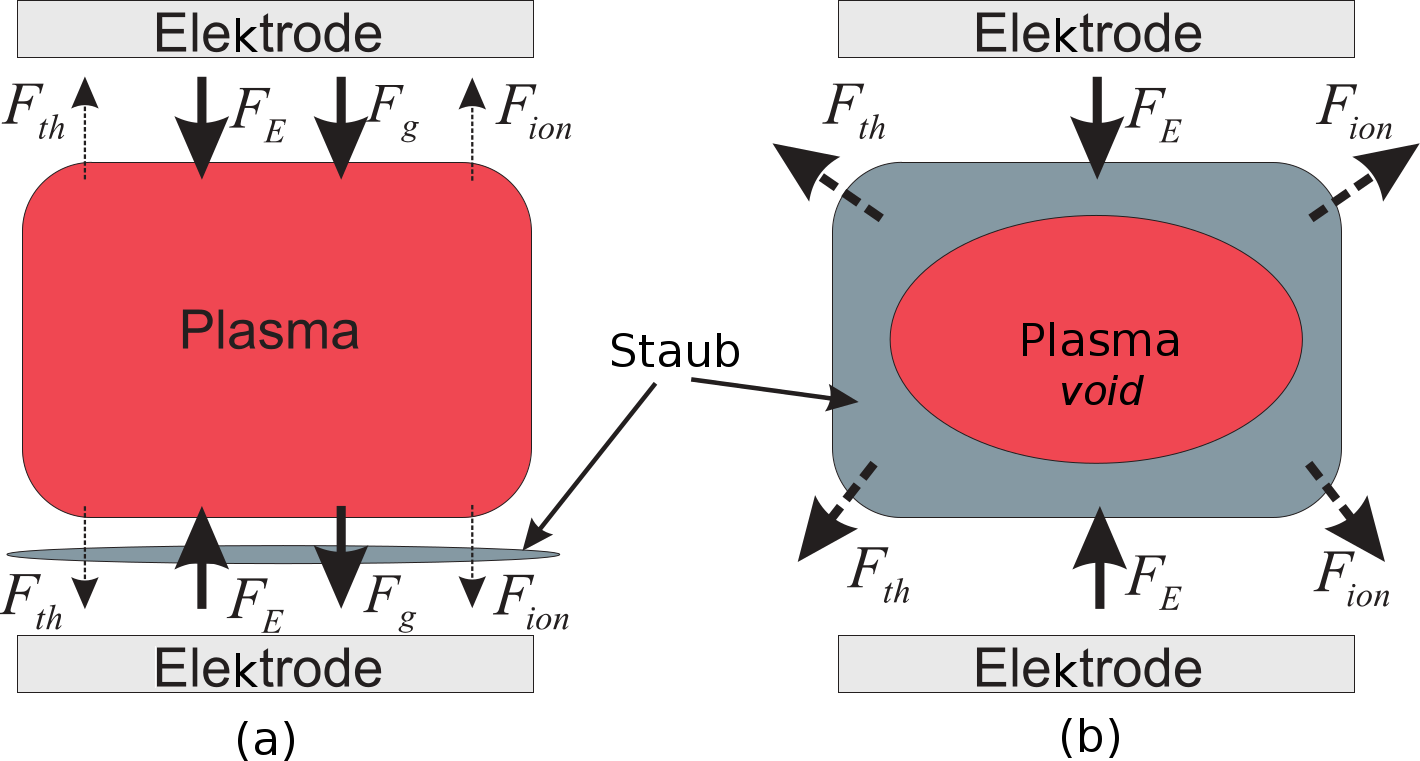
\includegraphics[width=\textwidth,height=0.5\textwidth]{figs/directionsofforcesandtrappingmelzer.png}
						\caption{Schemata für dein Einfang von Staub mit (a): $a\approx\unit[\tenpo{-5}]{m}$ (b): $a\approx\unit[\tenpo{-9}]{m}$ bzw. unter Mikrogravitation. Es wurden die wichtigsten Kräfte und deren Richtungen eingezeichnet.}
						\label{img:kräfterichtungen}
					\end{figure}
					
				
		\subsection{Finite Yukawa-Cluster}\label{subsec:yukawaclust}
					
		\subsection{Coulomb-Kristallisation}\label{subsec:coulombkristall}			
					
	\newpage
	
	\section{Durchführung}\label{sec:durch}
	
	\newpage
	
	\section{Auswertung}\label{sec:auswert}
	
	\newpage
	
	\section{Literatur}\label{sec:lit}
	
		\bibliography{all_melzer.bib}
		\bibliographystyle{unsrt}
	
	\newpage
	
	\section{Anhang}\label{sec:anhang}
	
%		\subsection{Abkürzungsverzeichnis}\label{subsec:abkurz}
%		
%			\begin{acronym}
%				
%			\end{acronym}
	
\end{document}
